% This LaTeX document needs to be compiled with XeLaTeX.
\documentclass[11pt]{article}
\usepackage[utf8]{inputenc}
\usepackage{ucharclasses}
\usepackage{amsmath}
\usepackage{amsfonts}
\usepackage{amssymb}
\usepackage[version=4]{mhchem}
\usepackage{stmaryrd}
\usepackage{multirow}
\usepackage{graphicx}
\usepackage[export]{adjustbox}
\graphicspath{ {./images/} }
\usepackage{hyperref}
\hypersetup{colorlinks=true, linkcolor=blue, filecolor=magenta, urlcolor=cyan,}
\urlstyle{same}
\usepackage{polyglossia}
\usepackage{fontspec}
\setmainlanguage{english}
\setotherlanguages{hindi}
\newfontfamily\hindifont{Noto Serif Devanagari}
\newfontfamily\lgcfont{CMU Serif}
\setDefaultTransitions{\lgcfont}{}
\setTransitionsFor{Hindi}{\hindifont}{\lgcfont}

\begin{document}
Credit Risk Analysis and the Bankruptcy Process

Because much of the private credit market is below investment grade, it is imperative that investors understand how to value these loans, as well as the work that is necessary to recover and protect assets in the case of a bankruptcy filing.

\section*{Credit Ratings, Yields, and Financial Ratios}
Moody's, S\&P, Fitch, and other rating agencies are paid by borrowers to assign ratings to bond issues and large loans. Investors rely heavily on these ratings to understand the credit risk of issues and to assign credit spreads to loans and bonds. Debt rated as investment-grade (such as Moody's Baa and above, S\&P BBB and above) is expected to have very low default rates, and therefore, lower credit spreads. With a sovereign debt yield of $4 \%$ and an investment-grade credit spread of $1 \%$, an A-rated bond would have a yield of $5 \%$, regardless of the coupon rate of the security. Debt rated as below-investment-grade is expected to have higher default rates and higher credit spreads. With a sovereign debt yield of $4 \%$ and a credit spread of $3 \%$, a B-rated bond would have a yield of $7 \%$, regardless of the coupon rate of the security.

Of course, most transactions in the private credit market, especially smaller loans with a single lender, are not rated by the credit ratings agencies. Investors can estimate the ratings that might be assigned by a rating agency by studying the balance sheet and income statement of the borrower. Once investors understand the credit risk, they can assign a credit spread to the unrated debt. As the debt gets more risky and more likely to default, the implied credit rating declines and the interest rate charged to the borrower increases. Most borrowers in the private credit market are unrated, but the implied credit rating methodology would classify many of these borrowers as having a credit rating of $B$.

Ratings agencies consider a number of variables when rating the credit quality of a borrower. Less-risky borrowers have higher profit margins, higher assets, lower debt, and lower interest expense. Businesses with lower revenue volatility and lower profit volatility are also regarded as less likely to default. The next exhibit illustrates the relations between ratings, credit risk, and two key financial ratios (interest coverage and leverage).

\begin{center}
\begin{tabular}{|c|c|c|c|c|c|}
\hline
\multicolumn{2}{|c|}{\multirow{2}{*}}{कi} &  & \multicolumn{2}{|c|}{Moody's} & \multirow[b]{2}{*}{Low} \\
\hline
 &  & S\&P's/Fitch & \begin{tabular}{c}
EBITA/Interest \\
Expense \\
\end{tabular} & Debt/EBITDA &  \\
\hline
\multirow{5}{*}{
\includegraphics[max width=\textwidth]{2024_04_10_a4f1ca289b861eaba170g-2(2)}
} & Aaa & AAA & 11.5 & 1.9 & \multirow{10}{*}{
\includegraphics[max width=\textwidth]{2024_04_10_a4f1ca289b861eaba170g-2(1)}
} \\
\hline
 & $\mathrm{Aa}$ & AA & 13.9 & 1.8 &  \\
\hline
 & A & A & 10.7 & 2.3 &  \\
\hline
 & Baa & BBB & 6.3 & 2.9 &  \\
\hline
 & $\mathrm{Ba}$ & $\bar{B} \bar{B}$ & 3.7 & $3 . \overline{7}$ &  \\
\hline
\multirow{5}{*}{
\includegraphics[max width=\textwidth]{2024_04_10_a4f1ca289b861eaba170g-2}
} & B & B & 1.9 & 5.2 &  \\
\hline
 & Caa & $\mathrm{CCC}$ & 0.7 & 8.1 &  \\
\hline
 & $\mathrm{Ca}$ & $\mathrm{CC}$ &  &  &  \\
\hline
 & $\mathrm{C}$ & C &  &  &  \\
\hline
 & D & D &  &  &  \\
\hline
\end{tabular}
\end{center}

\section*{Leverage and Debt Coverage Ratios Vary by Credit Rating}
Source: Moody's Financial Metrics.

For example, the high-yield borrowers illustrated in the exhibit Leverage and Debt Coverage Ratios Vary by Credit Rating exhibit above typically have interest coverage ratios (such as EBITA/interest expense ratios) below 3.7, meaning that the annual cash flow of the company is less than 3.7 times the annual interest expense paid on all borrowings. In contrast, investment-grade borrowers may have interest coverage ratios of 6 to 12 times. Leverage ratios are also very important, as high-yield borrowers have average debt levels at least 3.7 times EBITDA, whereas investment-grade borrowers have leverage ratios closer to 2 to 3 times. A complete listing of 11 financial ratios, as excerpted in the exhibit above, and their link to credit ratings is available online from Moody's Financial Metrics. ${ }^{1}$ Moody's Financial Metrics Key Ratios by Rating and Industry for Global Non-Financial Corporates, December 2016. Private credit investments may have even wider credit spreads than found using this implied credit rating method, as the illiquidity of the investment and the value added to the borrower are greater than is found in the public bond market.

\section*{Credit Spreads and Credit Risk}
One of the ways to analyze the fixed-income market is by the size of the credit spread observed on a given debt issue, ranging from safer investment-grade debt to riskier noninvestment-grade debt. A credit spread is the excess of the yield on a debt security with credit risk relative to the yield on a debt security of similar maturity but no credit risk.

An investment-grade credit spread is the amount of yield on an investment-grade debt security relative to a sovereign debt with comparable maturity demanded for investing in firms that have modest default risk. As investors move from the sovereign debt or risk-free level of interest rates into investment grade, they take on that additional amount of credit risk for which investors require compensation, which was under 100 basis points in the United States during 2021. The investment-grade market has relatively low interest rates because these issues have a low probability of default, as the debt is backed by a larger number of assets and dependable cash flows compared to the debt load of the firm.

However, there is often a tremendous difference between the yields of investment-grade debt and noninvestment-grade debt. This noninvestment-grade debt is also termed high-yield, speculative, or junk bonds. A company with lesser assets or lesser cash flows or a greater volatility of financial results may be determined to be a speculative-grade issuer, meaning that they would pay the higher interest rates required of below-investment-grade issuers. Firms in the high-yield or speculativegrade category will be charged higher borrowing costs, as they have a significantly higher probability of default, meaning that they might not pay their principal and\\
interest as scheduled. Sometimes the defaults are not driven by the failure to pay principal and interest, but rather by the failure to maintain covenants that might require the company to maintain a given level of cash flows or assets.

It's hard to estimate a yield curve for long-term high-yield debt, especially going out for very long maturities, because investors and borrowers may not want to contract for 30 years when the borrower (company) has a highly questionable ability to repay that loan due to concerns by lenders of high risk and concerns by borrowers of high costs. As a result, high-yield bonds tend to be issued with much shorter maturities. At year end 2021, the credit spread between US Treasuries and high-yield bonds was over 3.4\%, which means that investors could earn more than double the amount of interest on the high-yield bonds than they could on US Treasury bonds. Of course, high-yield issuers don't have the same ability to make coupon and principal payments as a sovereign issuer, which justifies the higher interest rate sought by investors to compensate for the increased credit risk, as losses from defaults offset part of the higher interest rate.

Session 6.2, Credit Risk and Credit Derivatives on credit derivatives discusses credit spreads in detail, including important models of credit spreads. Credit spreads depend on default probabilities, expected losses given default, and various potential risk premiums.

\section*{Credit Risk and the Probability of Default}
A relatively low spread of 100 basis points between sovereign debt and investment-grade issuers may be explained by the relatively minimal defaults on investmentgrade issues. This is the safest type of corporate debt, because even when the business cycle is getting rough, default rates on investment-grade debt don't reach $1 \%$. Thus, a credit spread of 100 basis points between sovereign debt and investment-grade debt is often viewed as sufficient to compensate investors for expected credit losses and systematic risk.

Global Default Rates: Investment-Grade Versus Speculative-Grade

\begin{center}
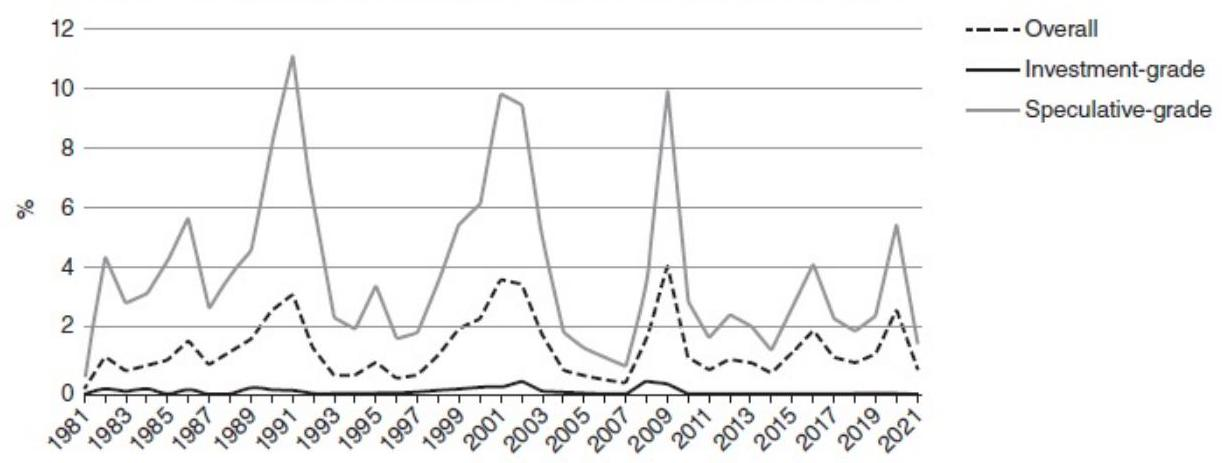
\includegraphics[max width=\textwidth]{2024_04_10_a4f1ca289b861eaba170g-3}
\end{center}

\section*{The Cyclicality of Global Default Rates}
Sources: S\&P Global Ratings Research and S\&P Global Market Intelligence's CreditPro .

Copyright $\odot 2022$ by Standard \& Poor's Financial Services LLC. All rights reserved.

The Cyclicality of Global Default Rates exhibit above shows the cyclicality of these markets and how extreme the losses on the speculative-grade, high-yield, or junk bond issues can be. The default rate on high-yield bonds actually exceeded 9\% three times in the past 30 years (around 1990, 2001, and 2008). A credit spread of 3 or $4 \%$ might not be sufficient to compensate for the losses at the bottom of the credit cycle. Default rates vary with the economy: the default rate can be very low for a long period of time when the economy is strong and very high during times of economic or financial crisis. The question is whether a credit spread of, say, $3.5 \%$ at the issue date of new debt will be sufficient to pay for expected default losses and increased risk over the life of the debt issue.

\section*{Covenants}
The Commercial Mortgages lesson in Section 3.4, Real Estate Assets and Debt, introduces covenants and other terms regarding default risk analysis. Covenants are promises made by a debtor to the creditor that strengthen the perceived credit quality of the obligation. Loan covenants may be required by creditors to protect their interests, or they may be offered by debtors to negotiate better terms. The types of bond covenants have been known to affect credit risk. For example, a factor that has driven the size of the distressed market in the past has been the proportion of loans that are covenant-light (cov-lite) loans. Covenant-lite loans are loans that place minimal restrictions on the debtor in terms of loan covenants. In 2016, over half of European loans were covenant-lite, compared to just $5 \%$ in 2007 , while more recently over three-quarters of US loans were covenant-lite. As the strength of covenants declines, the likely default rates rise and the likely recovery rates decline. Wigglesworth (2018) quotes Moody's estimates of these declines in recovery rates given the demise of covenants, with the recovery rate on first-lien debt perhaps falling from a historical average of $77 \%$ to $43 \%$, while second-lien recoveries could decline from $43 \%$ to $14 \%$.

An indenture is the contract between the borrower and the lender that sets out the terms of the borrowing. These terms may include the interest rate, maturity date, face value, and the schedule of payments, as well as covenants. Affirmative covenants are requirements for the borrower to comply with, such as to maintain a debt service coverage ratio that requires a minimum income relative to the size of the current year principal and interest payments. Ideally, investors would require that the cash flow of the company be at least twice what the firm owes in current-year debt payments, giving a cushion in order for the borrower to service their debt payments as well as to reinvest in their business. Under these affirmative covenants, the firm must disclose their financial results to prove compliance with covenants, such as the need to maintain a given level of assets relative to their debt burden or a specific level of cash flow or earnings before interest, taxes, depreciation, and amortization (EBITDA) relative to their annual interest expense. Negative covenants, or prohibitions on actions of the borrower, might prevent the company from increasing their debt load or issuing any new debt with seniority to the current first-lien debt issues.

When a borrower fails to maintain either the affirmative or the negative covenants, they can be in technical default on the loan. Upon that default, the creditors can step in and take action to accelerate the loan by requiring immediate repayment, restructure the loan at a higher borrowing cost, move to seize collateral, or force the borrower into bankruptcy proceedings.

Covenants are in the bond indenture in order to protect the lenders and/or lower the borrowing cost of the borrower. Covenants increase the security of a loan, requiring the company to meet certain financial targets and submit to oversight by the lender. As investment capital continues to flow into the increasingly\\
competitive private credit market, there is an increasing amount of covenant-light issuance in both the high-yield bond market and the private debt market, transferring the balance of power toward the borrowers.

Another distinction between covenants is incurrence covenants versus maintenance covenants. Incurrence covenants typically require a borrower to take or not take a specific action once a specified event occurs. For instance, if an incurrence covenant states that the borrower must maintain a limit on total debt of five times EBITDA (earnings before interest, taxes, depreciation, and amortization), the borrower can take on more debt only as long as it is still within this constraint. A borrower that breaches this covenant by incurring additional debt is in default of the covenant and the loan. However, if the borrower found itself above the five times EBITDA limit simply because its earnings and cash flow had deteriorated (without having incurred additional debt), it would not be in violation of the incurrence covenant and would not be in default. Cov-lite loans have bond-like incurrence covenants, much like high-yield bonds.

Maintenance covenants are stricter than incurrence covenants in that they require that a standard be regularly met to avoid default. Returning to the previous example of a covenant wherein the debt is limited to five times EBITDA, in the case of a maintenance covenant, the borrower must pass this test each and every quarter, regardless of whether it added more debt or its earnings and cash flow deteriorated. Thus, the covenant would be triggered if the borrower's earnings and cash flows eroded, even if the firm did not issue new debt. Clearly, maintenance covenants are much stronger than incurrence covenants. Without maintenance covenants, lenders do not have the ability to step in at an early stage to reprice risk, restructure the loan, or shore up collateral provisions.

\section*{Five Ways Covenants Can Control Risk}
Antczak, Lucas, and Fabozzi (2009) explain five ways in which covenants can control risk for lenders: ${ }^{2}$ Antczak, Stephen J., Douglas J. Lucas, and Frank J. Fabozzi. 2009. Leveraged Finance: Concepts, Methods, and Trading of High-Yield Bonds, Loans, and Derivatives. Hoboken, NJ: John Wiley \& Sons.

\begin{enumerate}
  \item Preservation of collateral: Because the value of the collateral is key to both the quality of the loan and the eventual recovery rate upon distress, lenders can control risk by limiting the size of the loan relative to the value of the firm and the value of the collateral. In many cases, lenders may require a maximum loanto-value ratio of $50 \%$ for inventory, $60 \%$ for property, plant, and equipment, and $80 \%$ for receivables. Senior secured loans should be of a limited size, perhaps half of the enterprise value of the firm. Finally, each asset should be pledged as collateral to only a single lender, which should go without saying.

  \item Appropriation of excess cash flow: Lenders are protected when the uses of corporate cash are limited. Many lenders require the majority or the entirety of the value of asset sales and new debt to be paid to the debt holders rather than to the equity holders. Increasing the debt load while liquidating assets reduces the value of the firm, so paying the proceeds from those transactions to equity holders reduces the security of the debt and increases the risk of the debt.

  \item Control of business risk: There is an inherent conflict between stockholders and bondholders. When the company prospers, the equity holders can experience large gains, whereas lenders earn principal and interest as contracted. When the company becomes distressed, the bondholders have a downside risk much larger than their upside return potential. Simply, the stockholders are long a call option on the firm's assets and the bondholders are therefore short a put option on the assets. This conflict leads to equity holders wishing to undertake risky projects when the firm is approaching distress, because the upside risk benefits the equity holders and hurts the bondholders. Therefore, it is in the best interest of the lenders to limit the types and sizes of investments, mergers, and debt that the firm can undertake.

  \item Performance requirements: Under negative covenants, the company must maintain strong ratios of assets and cash flow relative to the debt and interest burden of the firm. Capital expenditures may need to be limited in order to maintain compliance with the requested financial ratios.

  \item Reporting requirements: Under affirmative covenants, the company needs to report financial results to lenders, including other material information regarding projections of revenues and expenses, litigation, and regulatory issues.

\end{enumerate}

Consider the case of the 2018 leveraged buyout by Refinitiv, which purchased the data division of Thomson Reuters. Some analysts noted that the high-leverage multiple and weak covenants in this deal made it especially likely for this company to become distressed and could mark the beginning of the end of a credit cycle with increasingly borrower-friendly terms. There were three especially concerning nonstandard terms in this deal. First, the borrowers could prepay the unsecured bonds before the secured debt, meaning that cash flows are potentially going to the bottom of the capital structure when they are typically directed toward the top of the capital structure. Second, the company could be sold without the contractual requirement of paying off the debt, although typical transactions would require the buyer of a firm to secure financing of their own at terms that made sense at the time of the buyout. Third, and perhaps most concerning, is that there is not a limit on the cash that can be paid to equity holders, even when the borrower is not servicing their debt. It is certainly not a standard risk management practice to allow large dividends to be paid to the equity holders at the bottom of the capital stack when payments are delinquent to the debt holders at the top of the capital stack.

\section*{Capital Structure and Priority}
The capital structure, or capital stack, shown in the Priority of Claims in the Capital Structure exhibit, is the mix of equity and debt in any given firm. The riskier parts of the capital structure, such as equity, have a higher expected return, and the safest parts of an investment, such as secured and first-lien debt, should have a lower expected return. The lower-risk investments at the top of the capital structure may have a claim to a specific asset, such as a mortgage on a building, meaning that this loan has to be paid back before any other obligation of the firm.

\begin{center}
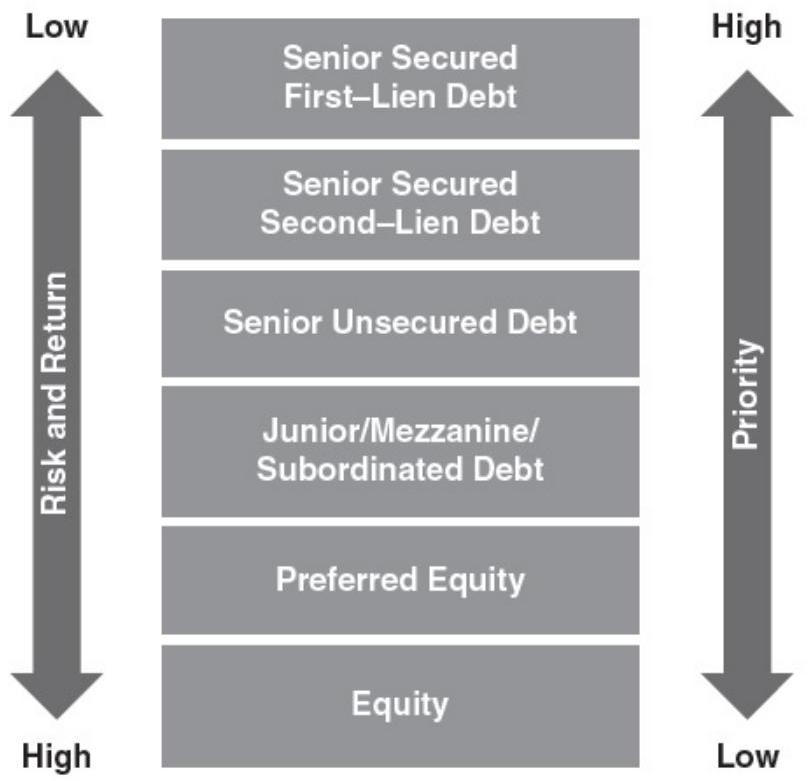
\includegraphics[max width=\textwidth]{2024_04_10_a4f1ca289b861eaba170g-5}
\end{center}

\section*{Priority of Claims in the Capital Structure}
Loans and secured borrowings typically have the highest credit quality, the highest claim or priority to assets in the case of a bankruptcy, and the lowest potential return. Next in line come bonds and unsecured debt with lower recovery rates and higher potential returns. Junior, mezzanine, subordinated, and convertible debt sit in the middle of the capital structure. These are debts of the firm, but each has a lesser claim to cash flows and assets than seen in the senior secured and first-lien debt. These issues in the middle of the capital structure are riskier than the senior debt and are likely to have a higher interest rate. The amount of risk an investor takes should be commensurate with the yield the investor is going to earn. As one invests in riskier and riskier parts of a given company, or as one invests in riskier or riskier companies, one should have a higher level of return expectations.

Equity and preferred issues sit at the bottom of the capital stack. These investors have the lowest claim on assets of the distressed firm, but the highest potential return on investment when the firm performs well.

The capital structure of the firm can change over time, such as when there's a debt-equity swap, where the proceeds of a debt issue are paid to the equity holders through dividends or stock buybacks. Increasing borrowing and repurchasing stock changes the capital structure of the firm and increases the debt-to-equity ratio.

Historically, senior debt issues had lower interest rates and a higher place in the capital stack. If borrowers needed to access more debt capital than allowed in the senior debt market, they would need to turn to the subordinated debt market to access that extra debt capital at a much higher interest rate.

In recent years, there has been substantial growth in the unitranche debt market, in which a large piece of debt is issued that includes both senior and junior debt at a blended interest rate in a single debt issue. The unitranche structure could bring benefits for both borrowers and lenders. Borrowers have a less complex capital structure and may be willing to pay a higher interest rate on a unitranche borrowing for this convenience. Lenders may also prefer a less complex capital structure, because it avoids conflicts between creditors and makes workouts much easier, as the lender of the junior debt is also the lender of the senior debt. Unitranche debt has become so popular that it appears that mezzanine lending is declining due to the rise of direct lending and unitranche structures.

\section*{Recovery Rates}
When a firm defaults, they may not be able to pay their principal and interest as scheduled or the firm may fail to comply with one or more of their covenants, in that their cash flow or asset value drops to a point where it appears that they're not able to service the debt. Our first concern is the default rate, which is the percentage of loans or bonds in our portfolio that have defaulted. Next, lenders are concerned about recovery rates.

The recovery rate is the portion of the face value of the debt that is paid back from the assets of the firm in a bankruptcy. In a liquidation bankruptcy, the lenders or the court have decided that this company is no longer a going concern. The business model of the company is not likely to earn cash flows that are sufficient to pay back the debt, even if that debt has been restructured. In a liquidation bankruptcy, the assets of the firm are distributed to creditors or sold with the proceeds being distributed. Firms are in default because their assets and cash flows are not sufficient to pay the liabilities of the firm.

A reorganization bankruptcy can make sense for a good company with a bad balance sheet. If the liabilities can be reduced or reorganized, the company could be profitable. If the firm simply had less debt, it would be able to be profitable going forward. In a reorganization bankruptcy, the firm can renegotiate any and all liabilities, such as union contracts, leases, pensions, and debt issues. With the assistance of the court, the borrower renegotiates all liabilities and seeks to change contracts in a way that allows the firm to continue its operations in a profitable manner.

First-lien term loans or secured bonds have the highest recovery rate, as those debt issues sit at the top of the capital structure as the safest investments likely recover the majority of the value of those assets in bankruptcy. Recovery rates have averaged $76 \%$ on first-lien loans, $56 \%$ on secured bonds, and $44 \%$ on senior unsecured bonds. Subordinated debt or junior debt will have lower recovery rates, often in the $20 \%$ to $30 \%$ range. In a reorganization, the senior debt holders often take a haircut, or a reduction in the amount owed, perhaps accepting new debt with a face value of $70 \%$ to $80 \%$ of the old debt, which is a haircut of $20 \%$ to $30 \%$ of the face value. Subordinated debt is often cancelled and converted into an equity stake in the newly reorganized firm, which hopefully is a going concern where the ongoing cash flows of the firm are no longer encumbered by the legacy liabilities.

At the bottom of the capital stack, the equity holders before bankruptcy typically lose their entire investment in a liquidation or a reorganization bankruptcy because the firm is in default and doesn't have the assets or the cash flow to pay their senior and junior debt in full. If the assets and the cash flow are insufficient to pay the senior debt and the junior debt, there are no assets left over for the equity holders. Equity is the riskiest part of the company's capital structure, where stockholders\\
who expect to make the highest return also can experience the largest losses. In a reorganization or in a liquidation bankruptcy, equity holders typically earn a zero recovery or experience a $100 \%$ loss of their capital.

\section*{Distressed Debt and the Bankruptcy Process}
Investing in below-investment-grade and distressed debt is inextricably linked with the bankruptcy process. Many distressed debt investors purchase the debt while the borrowing company is in the throes of bankruptcy. Other investors purchase the debt before a company enters into bankruptcy proceedings with the expectation of gaining control of the company through the bankruptcy proceedings. In either case, distressed investors need to be experts in bankruptcy procedures. This section illustrates issues involved in bankruptcy using US bankruptcy law. Some countries only have laws that allow for liquidations as a result of a bankruptcy filing, as reorganizations are not supported by the legal structure in all domiciles.

There are two major forms of US corporate bankruptcy: Chapter 7 and Chapter 11. Chapter 7 bankruptcy is when the assets of a firm are liquidated when a company is determined to no longer be a viable business. Essentially, the firm shuts down its operations and parcels out its assets to various claimants and creditors. The critical issue in Chapter 7 bankruptcies is the priority of claims: who gets paid first, who gets paid most, and which obligations are never repaid.

Chapter 11 bankruptcy is a reorganization that attempts to maintain operations of a distressed corporation that may be viable as a going concern. It therefore affords a troubled company protection from its creditors while the company attempts to work through its operational and financial problems. Generally, under a Chapter 11 bankruptcy, the debtor company proposes a plan of reorganization. A plan of reorganization is a business plan for emerging from bankruptcy protection as a viable concern, including operational changes. The plan includes how creditors and shareholders are to be treated under the new business plan. The claimants in each class of creditors are entitled to vote on the plan of reorganization. If all impaired classes of security holders vote in favor of the plan, the bankruptcy court conducts a confirmation hearing. If all requirements of the bankruptcy code are met, the plan is confirmed, and a newly reorganized company emerges from bankruptcy protection.

Thus, the sequence of events in a Chapter 11 bankruptcy centers on a plan of reorganization. The skeleton of the process is as follows:

\begin{itemize}
  \item The debtor company files for protection under Chapter 11.
  \item The bankruptcy court automatically stays, or suspends, all default notices from lenders.
  \item The debtor company exclusively has 120 days to develop and file a plan of reorganization.
  \item The debtor company then has another 60 days to convince creditors to accept the plan.
  \item If half of the number and two-thirds of the value of each class of claimants accept the plan, then court approval is sought through a confirmation hearing.
\end{itemize}

During the first 180 days after filing for protection, no other party of interest may file a competing reorganization plan. By giving the debtor company 120 days to propose its reorganization plan and another 60 days to persuade creditors, the bankruptcy code puts the emphasis on reorganization over liquidation and puts the debtor in the driver's seat, at least initially. After the exclusive period ends, any claimant may file a reorganization plan with the bankruptcy court. At this point, the process can become very acrimonious.

There are numerous variations and contingencies of the process. The following items provide introductions to some of the most important concepts involved in bankruptcy proceedings:

\begin{itemize}
  \item Classification of claims: Under the bankruptcy code, a reorganization plan may place a claim in a particular class only if such claim is substantially similar to the other claims in that class. For instance, all issues of subordinated debt by a company may constitute one class of creditor under a bankruptcy plan. Similarly, all secured bank loans (usually the most senior of creditor claims) are usually grouped together as one class of creditor. Finally, at the bottom of the pile is common equity, the last class of claimants in a bankruptcy.
  \item Prepackaged bankruptcy filing: Sometimes a debtor company agrees in advance with its creditors on a plan of organization before it formally files for protection under Chapter 11. Creditors usually agree to make concessions up front in return for equity in the reorganized company. The company then files with the bankruptcy court, submits a previously negotiated plan of reorganization, and quickly emerges with a new structure.
  \item Blocking position: A blocking position exists when a creditor or group of creditors holds more than one-third of the dollar amount of any class of claimants and utilizes those holdings to prevent a plan of reorganization. Recall that acceptance of a plan is usually predicated on a vote of each class of security holders, which requires support of two-thirds of the dollar amount of the claims in each class of creditors. Therefore, a single investor can obtain a blocking position by purchasing more than one-third of the debt in any class. A blocking position forces the other parties to negotiate with the blocking creditor.
  \item The cramdown: The bankruptcy code provides that a reorganization plan may be confirmed over the objection of any impaired class that votes against it as long as the plan (1) does not unfairly discriminate against the members of that class and (2) is fair and equitable with respect to the members of that class. This process within a bankruptcy is called a cramdown when a bankruptcy court judge implements a plan of reorganization over the objections of an impaired class of security holders (the plan is "crammed down the throats" of the objecting claimants). Cramdowns are usually an option of last resort when the debtor and creditors cannot come to an agreement. Bankruptcy courts have considerable discretion to determine what constitutes unfair discrimination and fair and equitable treatment for members of a class. In practice, cramdown reorganizations are rare. Eventually, the debtor and creditors usually come to some resolution.
  \item Absolute priority: An absolute priority rule is a specification of which claims in a liquidation process are satisfied first, second, third, and so forth in receiving distributions. Payments to employees, payments for taxes, and accounts payable generally take priority over payments to security holders. Senior secured debt holders (typically bank loans) must be satisfied first among security holders. The company's bondholders come next. These may be split between senior and subordinated bondholders. The company's preferred and common shareholders get whatever remains. As the company pie is split up, it is usually the case that senior secured debt is made whole and that subordinated debt receives some payment less than its face value, while the remainder of the company's obligations is transformed into equity in the reorganized company. Last, the original equity holders often receive nothing. Their equity is replaced by the new equity converted from the old subordinated debt. The ability of the court in the bankruptcy process to wipe out the ownership of existing shareholders and to transform the debt of senior and subordinated creditors into the company's new equity class is a key factor in distressed debt investing.
  \item Debtor-in-possession financing: When secured lenders extend additional credit to the debtor company, it is commonly known as debtor-in-possession financing (DIP financing). The borrower's desire in seeking DIP financing is clear: without additional credit, the borrower might not continue in business and would be forced to shut down. Creditors are often willing to grant DIP financing for a number of reasons. First, it keeps the debtor company afloat and gives it a chance to work out from under its debt load. Second, under bankruptcy law, DIP loans get priority over any forms of debt or financing incurred by the debtor before filing for bankruptcy under Chapter 11.
\end{itemize}

The Chapter 11 bankruptcy described above is applicable only in the US. Each country will have its own credit enforcement and bankruptcy regime. For example, in the US, companies in dire financial situation can choose between liquidation or reorganization bankruptcies. Most companies in the US choose reorganization bankruptcies. In contrast, most European jurisdictions historically only allowed liquidation bankruptcies. But the European Union is reforming their bankruptcy regime to also allow for reorganization bankruptcies, which will be in place in all member countries by $2022 .^{3}$ Extracted from \href{https://voxeu.org/article/eu-sinsolvency-reform}{https://voxeu.org/article/eu-sinsolvency-reform} The Asia Pacific region is geographically and politically vast. Thus, bankruptcy regime in the Asia Pacific region differs significantly from country to country in terms of procedures and terms. The different bankruptcy regimes create opportunities for distressed debt investors who can specialize in a particular legal system or region.


\end{document}